\documentclass[12pt]{article}
\usepackage{amsmath, amssymb}
\usepackage{graphicx}
\usepackage{listings}
\usepackage{xcolor}
\usepackage{hyperref}
\usepackage{geometry}
\geometry{margin=1in}

\title{Mars Exploration Environment: \\
A Logic-Based Autonomous Agent System}
\author{Mahla Entezari}
\date{Fall 2024}

\definecolor{codebg}{rgb}{0.95,0.95,0.95}
\lstset{
  backgroundcolor=\color{codebg},
  basicstyle=\ttfamily\small,
  frame=single,
  breaklines=true
}

\begin{document}

\maketitle

\begin{abstract}
This report presents the development of a Mars exploration simulation using a grid-based environment and a knowledge-based agent implemented via first-order logic (FOL). The environment includes hazards (holes), resources (goods), and a partially observable state space. The agent utilizes a deterministic depth-first search (DFS) strategy informed by logical inference rules to safely navigate and collect all resources. Visualization is implemented using Pygame, and agent decisions are grounded in formal logical expressions.
\end{abstract}

\section{Introduction}

Exploring hazardous and uncertain terrains such as those found on Mars requires agents capable of logical reasoning, partial observability handling, and safe decision-making. In this project, we simulate such an environment and propose a logical agent that models its behavior using a formal predicate logic system. The aim is to collect all resources (goods) while avoiding hazards (holes) in a grid environment.

\section{System Overview}

\subsection{Environment Structure}

The environment is a $H \times W$ grid initialized with:
\begin{itemize}
    \item A single agent at position $(0, 0)$ or randomized.
    \item Randomly placed \textbf{holes} (hazards).
    \item Randomly placed \textbf{goods} (collectible resources).
\end{itemize}

Each cell in the grid can be in one and only one of the following states:
\begin{itemize}
    \item Empty
    \item Contains a Hole
    \item Contains a Good
\end{itemize}

\subsection{Core Logical Constraints}

\begin{itemize}
    \item \textbf{State Exclusivity:}
    \[
    \forall c \in \text{Grid}, \left(
        \text{Hole}(c) \rightarrow \neg\text{Good}(c) \land \neg\text{Empty}(c) \land
        \text{Good}(c) \rightarrow \neg\text{Hole}(c) \land \neg\text{Empty}(c)
    \right)
    \]
    
    \item \textbf{Safe Movement:}
    \[
    \text{SafeMove}(d) \equiv \exists c \in \text{Adjacent}(d), \neg\text{Hole}(c)
    \]

    \item \textbf{Collect Good:}
    \[
    \text{CollectGood}(d) \equiv \exists c \in \text{Adjacent}(d), \text{Good}(c)
    \]

    \item \textbf{Termination:}
    \[
    \text{GameOver} \equiv \exists c, \left(\text{AtAgent}(c) \land \text{Hole}(c)\right) \lor \left( \forall c, \neg\text{Good}(c) \right)
    \]
\end{itemize}

\section{Agent Design}

\subsection{Logic and Policy}

The agent is governed by first-order logic predicates:
\begin{itemize}
    \item $A_1(b)$: Is there a hole in block $b$?
    \item $A_2(b)$: Is there a good in block $b$?
\end{itemize}

\textbf{Suitability Rule:}
\[
A_2(b) \lor \left( \neg A_1(b) \land \forall r \in \text{Neighbors}(b), \neg A_2(r) \right)
\]

This rule ensures the agent either:
\begin{enumerate}
    \item Moves toward goods directly.
    \item Chooses a safe unexplored cell when no immediate goods are detected.
\end{enumerate}

\subsection{DFS Strategy}

A recursive Depth-First Search is used. The agent:
\begin{itemize}
    \item Marks the current cell as seen.
    \item Evaluates all valid adjacent cells based on logical suitability.
    \item Recursively visits suitable and unseen neighbors.
    \item Backtracks if no progress is possible.
\end{itemize}

\section{Implementation Details}

\subsection{Environment Class}

Key methods of the \texttt{Mars\_Exploration\_ENV} class include:
\begin{itemize}
    \item \texttt{init\_grid()}: Randomly populates the grid.
    \item \texttt{get\_adjacent\_blocks()}: Returns adjacent states.
    \item \texttt{take\_action(action)}: Updates the agent's position.
    \item \texttt{update\_env()}: Pygame-based rendering.
\end{itemize}

\subsection{Agent Class}

From \texttt{agent.py}:
\begin{lstlisting}[language=Python, caption=Suitability Evaluation]
selected = block.isGood() or (
    not block.isHole() and 
    not self._disjuntion(call_method_on_objects(r_neig, "isGood"))
)
\end{lstlisting}

\subsection{Execution Entry}

\begin{lstlisting}[language=Python, caption=Main Agent Execution]
if __name__ == "__main__":
    env = Mars_Exploration_ENV(grid_h=15, grid_w=15, num_hol=20, num_good=20)
    agent = FOL_Agent(env)
    agent.dfs(agent.env.get_current_position(), agent.env.get_adjacent_blocks())
\end{lstlisting}

\section{Visualization}

Real-time interaction is visualized via \texttt{pygame}. The agent is a green circle, holes are brown, and goods are blue crystals.

\begin{figure}[h]
\centering
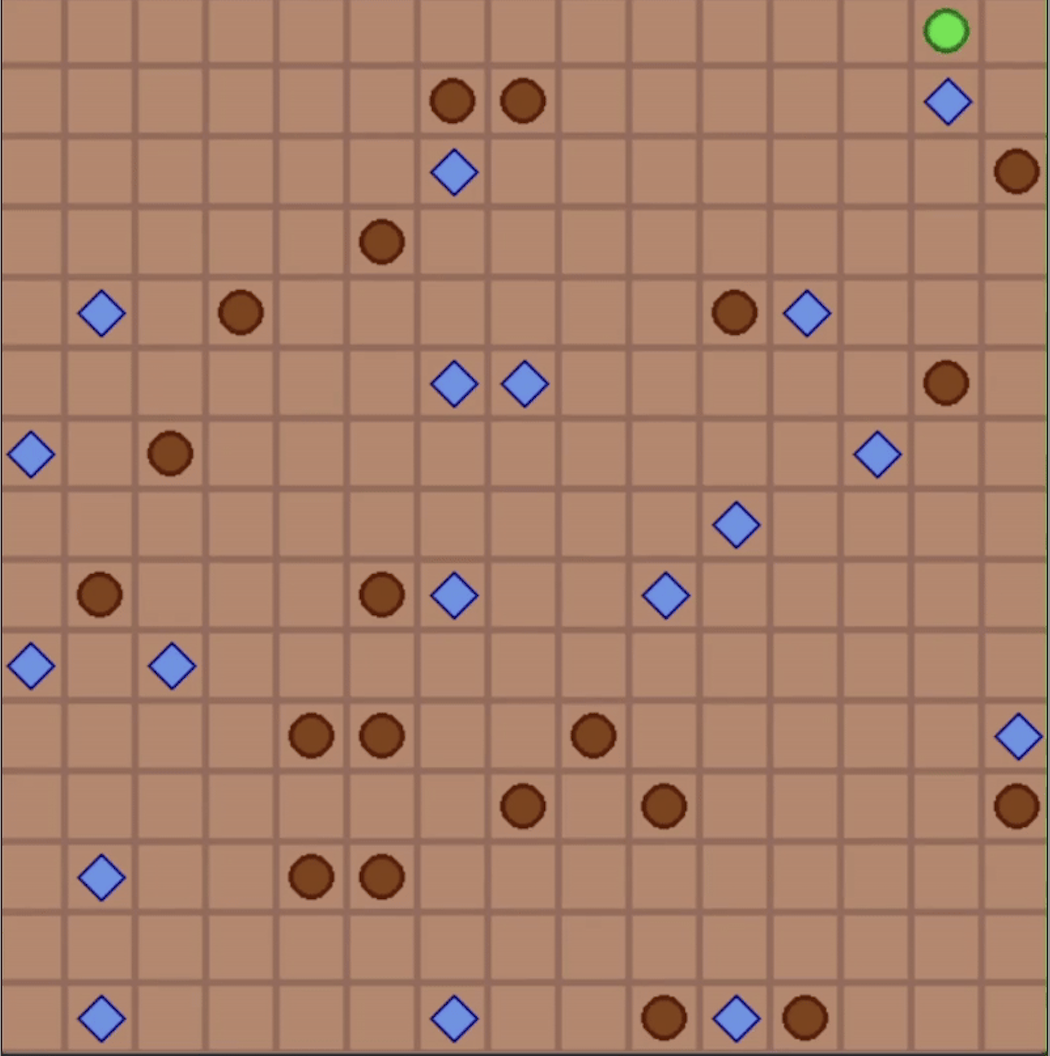
\includegraphics[width=0.5\textwidth]{start.png}
\caption{Start Simulation Snapshot}
\end{figure}

\begin{figure}[h]
\centering
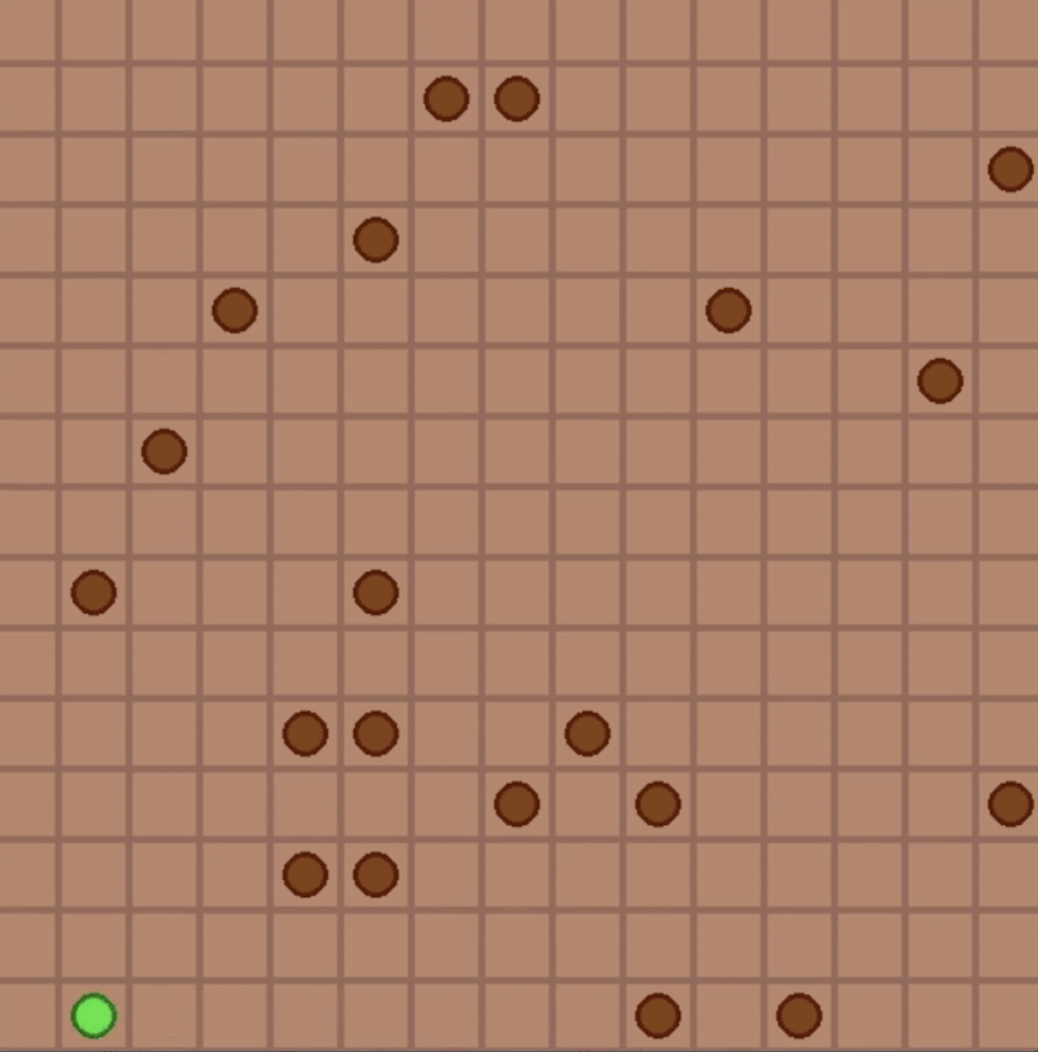
\includegraphics[width=0.5\textwidth]{end.png}
\caption{End Simulation Snapshot}
\end{figure}
\section{Conclusion}

This project demonstrates the application of first-order logic for autonomous exploration in a simulated Mars terrain. The agent's reasoning process ensures safe movement and efficient resource collection without prior map knowledge, relying entirely on local logical inference and recursive search.

\end{document}
